\documentclass[12pt]{article}
\usepackage[utf8]{inputenc}
\usepackage[T1]{fontenc}
\usepackage{geometry}
\usepackage{graphicx}
\usepackage{makeidx}
\usepackage{amsmath}
\usepackage{tabularx}
\geometry{margin=2.5cm}
\usepackage{fancyhdr}

\begin{document}
	
	\thispagestyle{empty}
	
	\begin{center}
		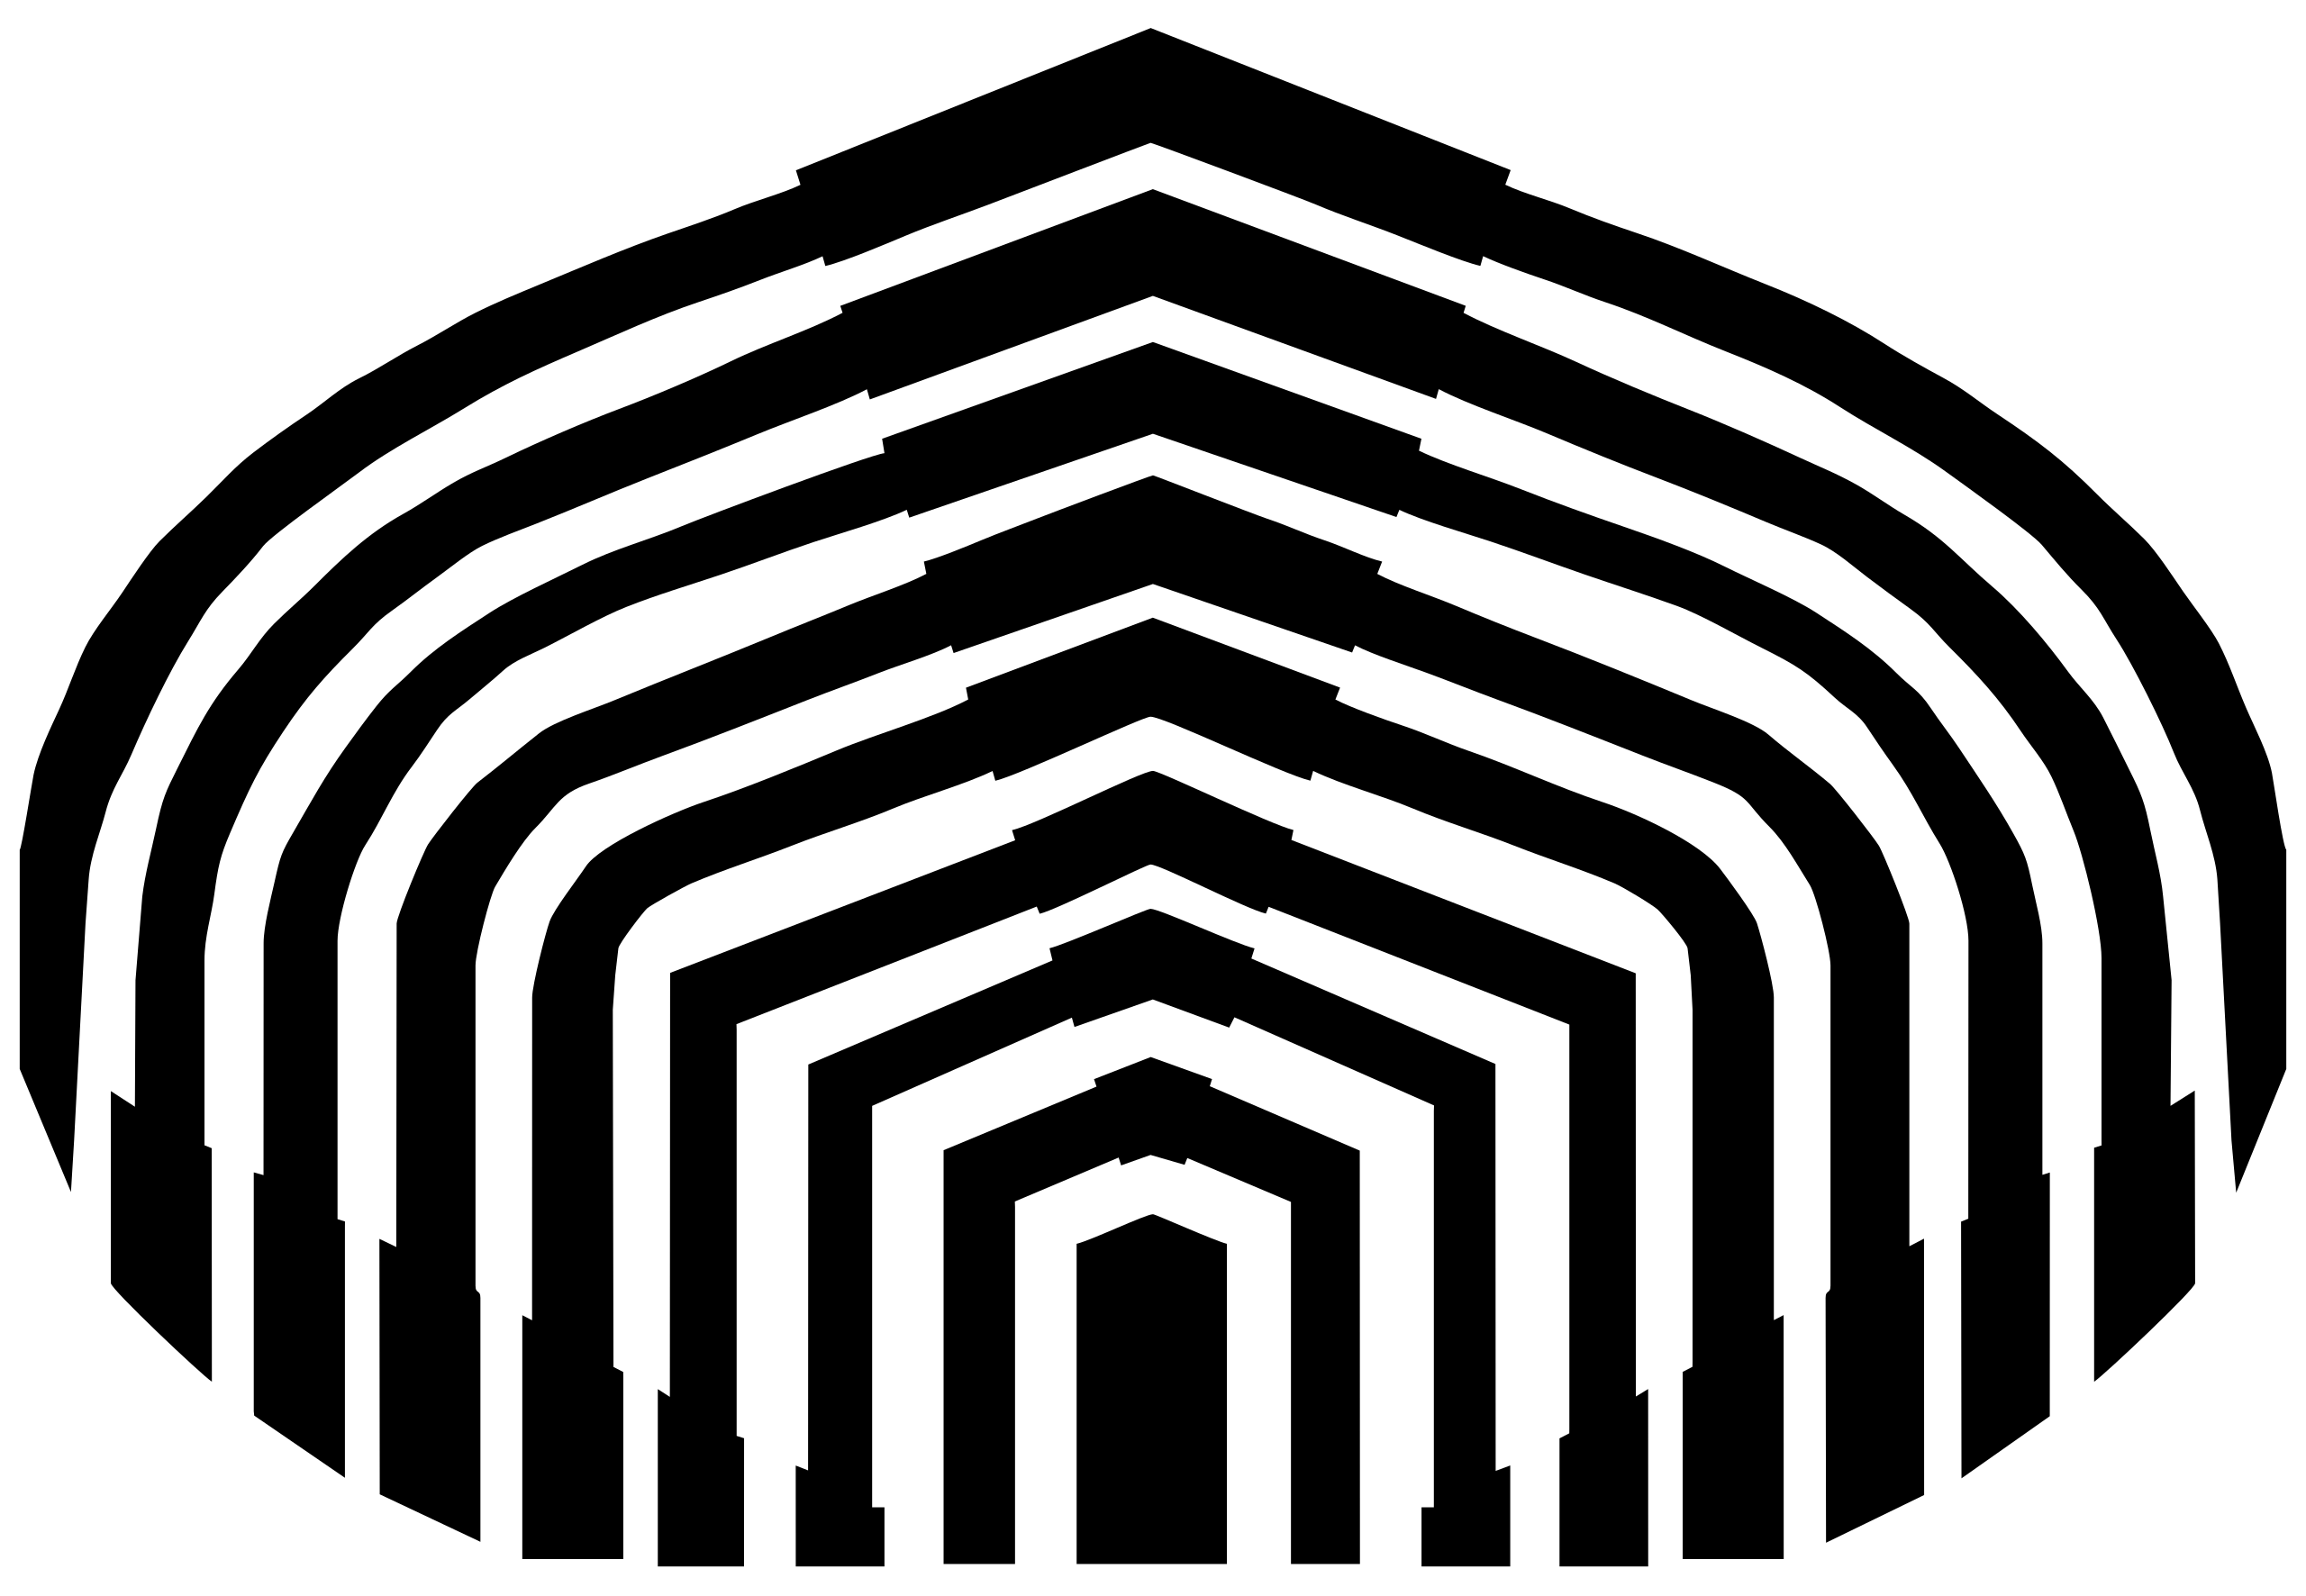
\includegraphics[width=3.1cm,height=2cm]{logo}\\
		UNIVERSIDAD SIMÓN BOLÍVAR\\
		DEPARTAMENTO DE ELECTRÓNICA Y CIRCUITOS\\
		EC1281 - LABORATORIO DE MEDICIONES ELÉCTRICAS\\
		SECCIÓN 1 - GRUPO 1\\
		
		\vspace{6cm}
		\textbf{\Large INFORME - PRÁCTICA \#9}\\
		MEDICIONES SOBRE CIRCUITOS ELECTRÓNICOS CIRCUITOS BÁSICOS DEL AMPLIFICADOR OPERACIONAL\\
	\end{center}
	
	\begin{flushleft}
		\vspace{9cm}
		\hfill Integrantes:\\
		\hfill {\large Luis Becerra - 1910557}\\
		\hfill {\large Lorena Rojas - 1910469}\\
	\end{flushleft}
	
	\newpage
	
	\pagenumbering{Roman}
        \setcounter{page}{2}
	
	\begin{center}
		\textbf{\large RESUMEN}\\
	\end{center}
	
	Los amplificadores operacionales (OPAM) son dispositivos electrónicos inmensamente versátiles que tienen una cantidad inmensa de aplicaciones. Dentro de los OPAM hay distintos modelos y cada uno será más conveniente para determinada tarea, uno de los más básicos es el UA741, un modelo versátil que se usa para distintas configuraciones y fue el escogido para esta práctica. Se detallan algunas de las características de dicho modelo de OPAM y algunas de las configuraciones más básicas para posteriormente ser probadas experimentalmente.
	
	\newpage
	
	\begin{center}
		\textbf{\large ÍNDICE}\\
	\end{center}
	
	\noindent \textbf{RESUMEN} \hfill \textbf{II}\\
	\noindent \textbf{ÍNDICE} \hfill \textbf{III}\\
	\noindent \textbf{MARCO TEÓRICO} \hfill \textbf{1}\\
	\noindent \textbf{METEDOLOGÍA} \hfill \textbf{3}\\
	\noindent \textbf{RESULTADOS} \hfill \textbf{5}\\
	\noindent \textbf{ANÁLISIS DE RESULTADOS} \hfill \textbf{17}\\
	\noindent \textbf{CONCLUSIONES} \hfill \textbf{22}\\
	\noindent \textbf{BIBLIOGRAFÍA} \hfill \textbf{23}\\
	
	\newpage
	
	\pagenumbering{arabic}
	
	\begin{center}
		\textbf{\large MARCO TEÓRICO}\\
	\end{center}
	
	El amplificador operacional UA741 es uno de los amplificadores operacionales más conocidos y utilizados en aplicaciones electrónicas. Tiene una amplia ganancia de voltaje, alta impedancia de entrada y baja impedancia de salida, lo que le permite amplificar señales débiles sin introducir distorsiones significativas. El UA741 es un amplificador de propósito general con una alta estabilidad y una amplia respuesta de frecuencia. Además, cuenta con una entrada diferencial y una salida de amplificación de voltaje, lo que lo hace adecuado para una variedad de aplicaciones, como amplificación, filtrado, sumador o comparador de señales.\\
	
	La respuesta de un amplificador operacional, como el UA741, puede variar según la frecuencia de la señal aplicada. En general, el UA741 tiene una respuesta de frecuencia plana en un rango amplio, lo que significa que puede amplificar señales de baja frecuencia y alta frecuencia de manera uniforme. Sin embargo, a medida que la frecuencia aumenta, la ganancia del amplificador puede disminuir gradualmente debido a la limitación de la velocidad de respuesta del dispositivo. Esta disminución en la ganancia a frecuencias más altas se conoce como respuesta en frecuencia de caída. Por lo tanto, es importante tener en cuenta las limitaciones de frecuencia al utilizar el UA741 en aplicaciones de alta frecuencia, donde se requiere una ganancia constante en todo el rango de frecuencia.\\
	
	El amplificador inversor es una configuración común y ampliamente utilizada. En esta configuración, la entrada de señal se aplica a través de una resistencia conectada al terminal negativo del amplificador operacional, mientras que la salida se toma del terminal de salida que está realimentada negativamente y en la línea de realimentación se coloca una resistencia que junto a la resistencia conectada a la entrada de la señal, determinarán la ganancia. La principal característica destacada de este amplificador es que proporciona una ganancia negativa y establecida por la relación de las resistencias en la configuración. Esto permite obtener una señal amplificada e invertida en la salida en comparación con la entrada. Su ganancia viene dada por:\\
	
	\begin{equation}
		\notag V_0 = -V_{ent}\frac{R_2}{R_1}
	\end{equation}\\

	El amplificador no inversor es otra configuración comúnmente utilizada. En esta configuración, la señal de entrada se aplica directamente al terminal no inversor del amplificador operacional, mientras que la señal de salida se toma del terminal de salida. La principal característica destacada de este amplificador es que proporciona una ganancia positiva y establecida por la relación de las resistencias en la configuración. Esto permite obtener una señal amplificada y no invertida en la salida en comparación con la entrada. La relación que determina la ganancia de nuestro circuito es:\\
	
	\begin{equation}
		\notag V_0 = \Big (1 + \frac{R_2}{R_1} \Big) V_{ent}
	\end{equation}\\

	El seguidor de voltaje, también conocido como buffer o amplificador de voltaje unitario, es una configuración utilizada para aislar y proporcionar una alta impedancia de entrada y baja impedancia de salida. En esta configuración, la señal de entrada se conecta directamente al terminal no inversor del amplificador operacional, y la señal de salida se toma del terminal de salida. La principal característica destacada de este amplificador es que proporciona una ganancia de voltaje de aproximadamente 1, lo que significa que la señal de salida es prácticamente idéntica a la señal de entrada, pero con una capacidad de conducción de corriente mejorada. Esto permite evitar la degradación de la señal al cargar circuitos de entrada sensibles, al mismo tiempo que proporciona una fuente de corriente capaz de alimentar circuitos de salida de baja impedancia. Se hace evidente que su ganancia es:\\
	
	\begin{equation}
		\notag V_0 = V_{ent}
	\end{equation}\\
	

	\newpage
	
	\begin{center}
		\textbf{\large METODOLOGÍA}\\
	\end{center}
	
	\begin{itemize}
		\item Primer circuito:\\
		
		Se realiza el montaje del amplificador inversor y las conexiones necesarias en la fuente DC. Luego, se conecta la entrada $V_i$ a $0V$ y se enciende la fuente DC para comprobar la alimentación del circuito y medir el voltaje de salida $V_0$, asegurándose de que el terminal negativo del voltímetro esté conectado a la tierra del protoboard. Si el voltaje de salida $V_0$ es de pocos $mV$ (voltaje de offset), se confirma que el amplificador operacional (OPAM) esté funcionando correctamente. En caso de que el voltaje de salida $V_0$ sea del orden del voltaje de saturación positivo o negativo, indica que el OPAM está dañado y debe ser reemplazado.\\
		
		Posteriormente, se mide con un voltímetro digital la amplitud de la ganancia de voltaje $(V_0/V_i)$ para los valores DC indicados. Se aplican los valores de voltaje DC utilizando un potenciómetro de $1k\Omega$ y se asegurará que la tierra de la fuente de $5V$ esté conectada al punto común de las dos fuentes de alimentación. En caso de utilizar valores negativos, se intercambian los cables en la fuente de $5V$. Se realizan las mediciones sin desconectar el potenciómetro del circuito para realizar los ajustes necesarios.\\
		
		A continuación, se aplica una señal sinusoidal al amplificador inversor con los valores indicados. Se observará simultáneamente en la pantalla del osciloscopio la señal de entrada y la de salida, midiendo voltaje y desfase. Se realiza una segunda medición de voltaje y desfase para $1V$ pico y $50kHz$.\\
		
		Luego, se procede a observar el efecto de saturación al aumentar la entrada a $2V$ y $1kHz$.\\
		
		Finalmente, se grafica la respuesta en frecuencia del amplificador operacional en la configuración de amplificador inversor. Se mide la amplitud de la ganancia de voltaje $(V_0/V_i)$ en un amplio rango de frecuencias. Se colocan señales sinusoidales de $1V$ de amplitud en la entrada, variando la frecuencia y verificando las amplitudes y frecuencias de las señales de entrada con el osciloscopio antes de realizar las mediciones.
		
		\item Segundo circuito:\\
		
		Una vez montado el amplificador no inversor, se procede a comprobar si el amplificador operacional funciona correctamente. Se realizan mediciones de la amplitud de la ganancia de voltaje $(V_0/V_i)$ para diferentes valores de voltaje DC de la entrada $V_i$, utilizando un potenciómetro para ajustar $V_i$.\\
		
		Luego, se aplica una señal sinusoidal al amplificador no inversor con los valores indicados. Se observará simultáneamente en la pantalla del osciloscopio la señal de entrada y la de salida, midiéndose el voltaje y el desfase.\\
		
		Se realiza una medición adicional de voltaje y desfase para una señal de $1V$ y $50kHz$.\\
		
		A continuación, se observa el efecto de la saturación al aplicar una entrada de $2V$ y $1kHz$.\\
		
		Por último, se mide la amplitud de la ganancia de voltaje $(V_0/V_i)$ en un amplio rango de frecuencias, utilizando una señal sinusoidal de amplitud de $1V$. Se agregan mediciones adicionales en las frecuencias de mayor interés alrededor de la frecuencia de corte.\\
		
		\item Tercer circuito:\\
		
		Una vez montado el seguidor de voltaje, se procede a comprobar si el amplificador operacional funciona correctamente. A continuación, se mide la amplitud de la ganancia de voltaje $(V_0/V_i)$ para los valores de voltaje DC indicados utilizando un voltímetro digital. Se aplican los valores de voltaje DC mediante un potenciómetro de $1k\Omega$ conectando sus extremos a la fuente de $15V$. Para valores negativos, se utilizará la fuente de $-15V$.\\
		
		Posteriormente, se aplica una señal sinusoidal al seguidor de voltaje con una señal de $10V$ pico y $10kHz$. Se observarán simultáneamente en la pantalla del osciloscopio la señal de entrada y la de salida, midiéndose el voltaje y el desfase. Asimismo, se realiza una medición de voltaje y desfase para una señal de $10V$ y $500kHz$.\\
		
		Finalmente, se lleva a cabo la medición de la respuesta en frecuencia del amplificador operacional en la configuración de seguidor de voltaje. Se mide la amplitud de la ganancia de voltaje $(V_0/V_i)$ en un amplio rango de frecuencias utilizando una señal de $1V$ de amplitud.\\
		
	\end{itemize}
	
	\newpage
	
	\begin{center}
		\textbf{\large RESULTADOS}\\
	\end{center}

	Presentando los resultados obtenidos del laboratorio:
	
	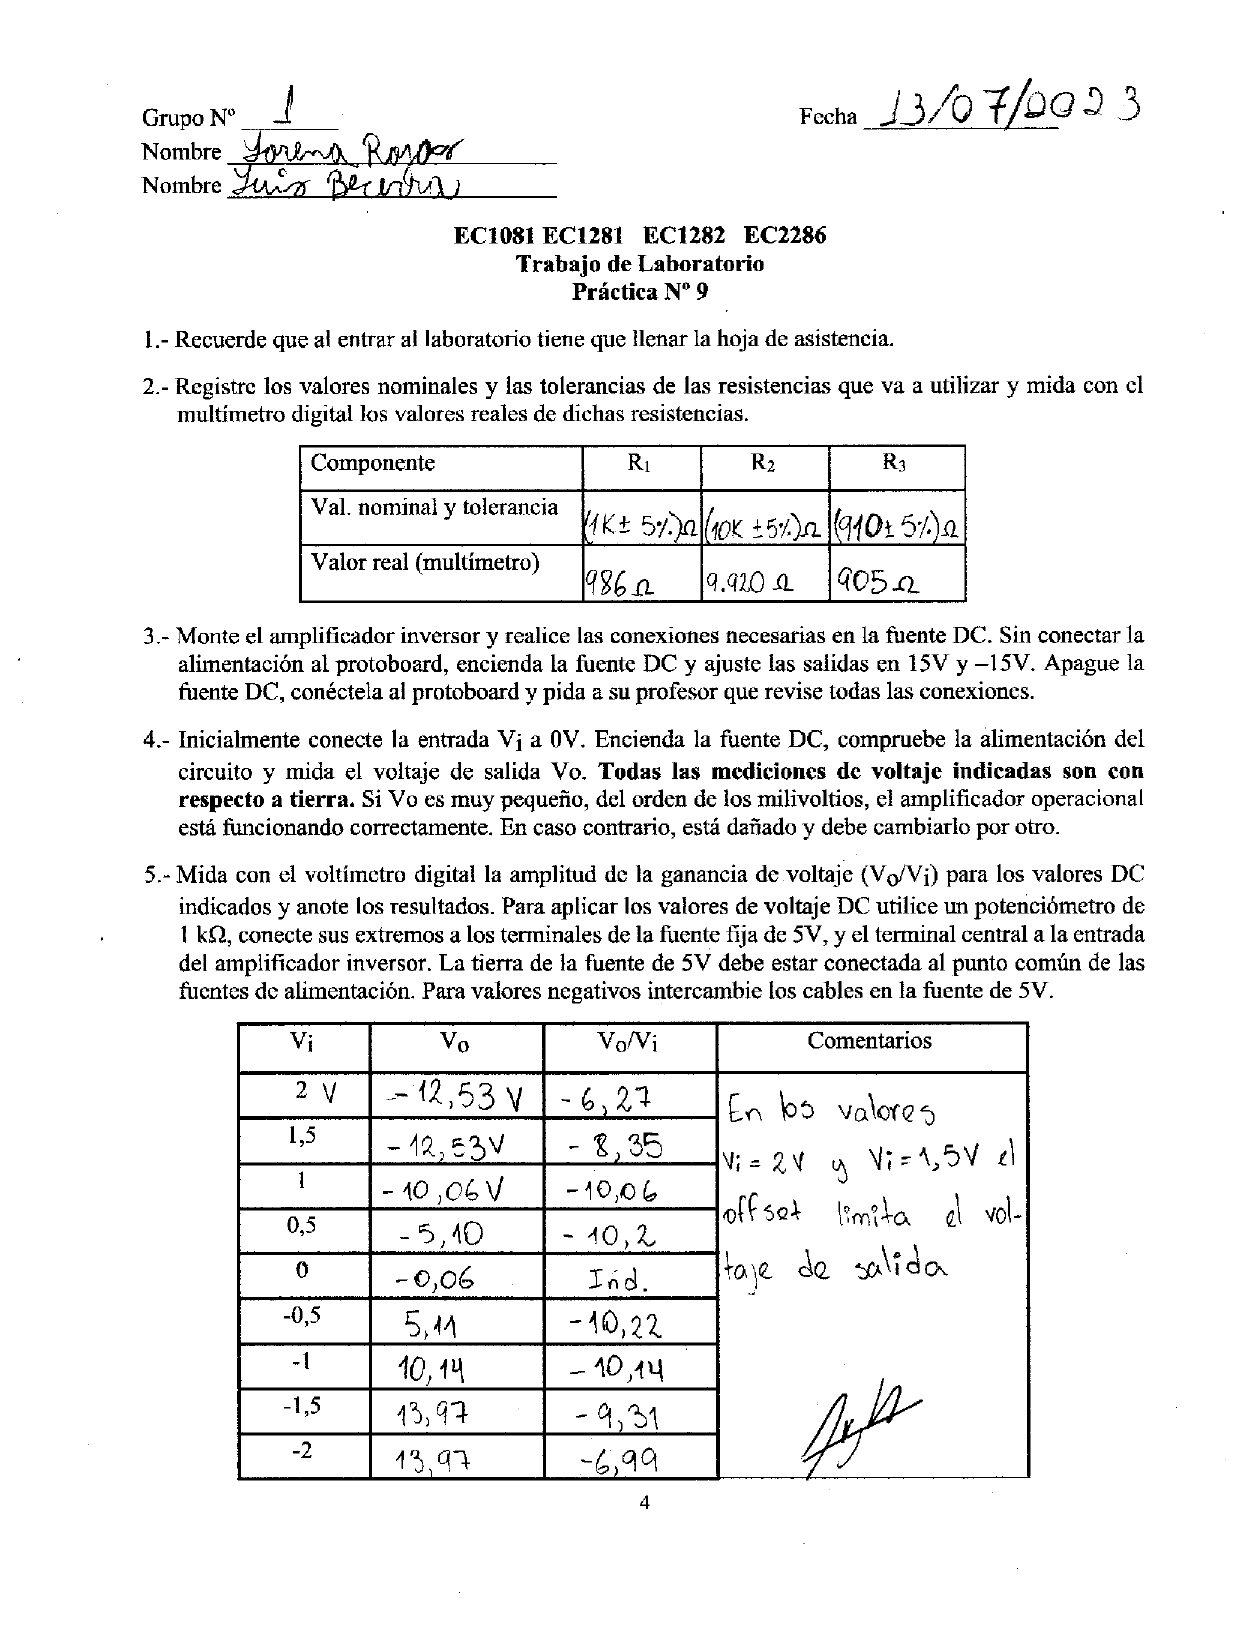
\includegraphics[width=16cm,height=21cm]{Img/lab_9_page-0001}\\
	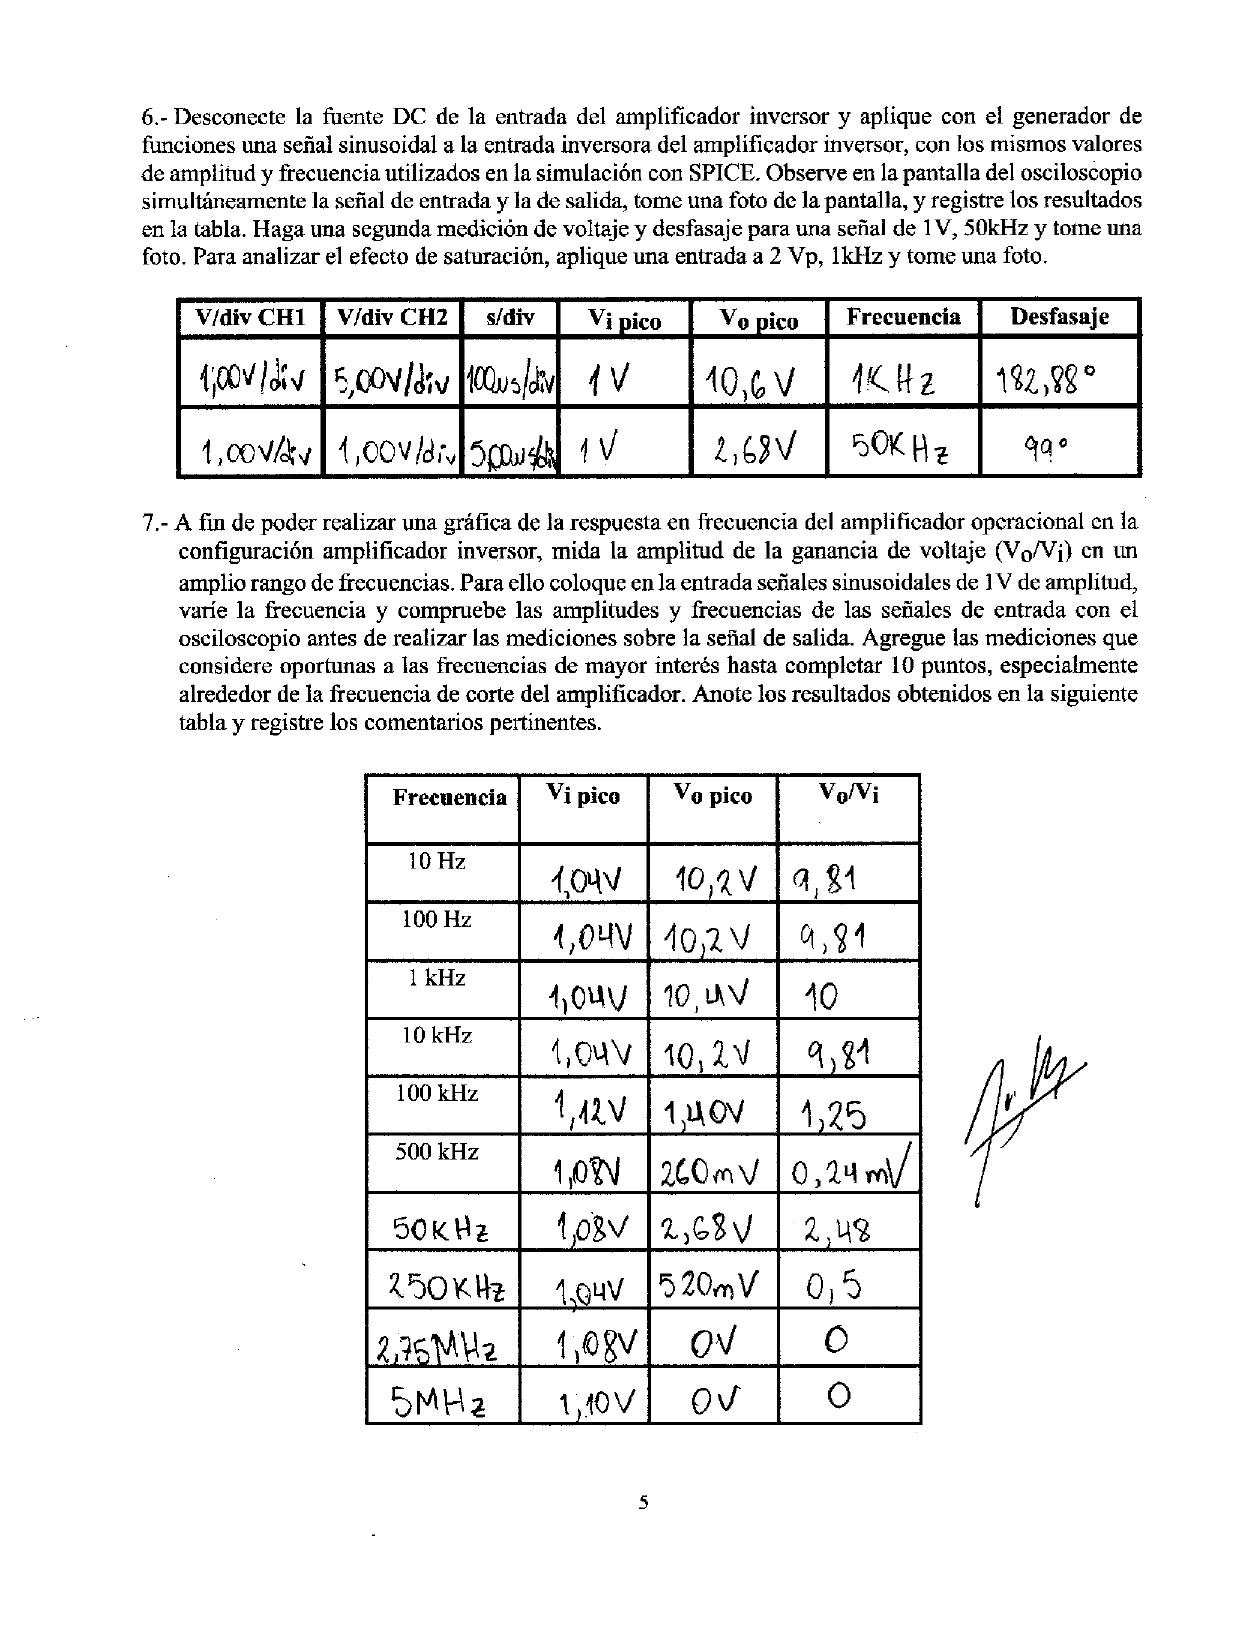
\includegraphics[width=16cm,height=21cm]{Img/lab_9_page-0002}\\
	
	\begin{center}
		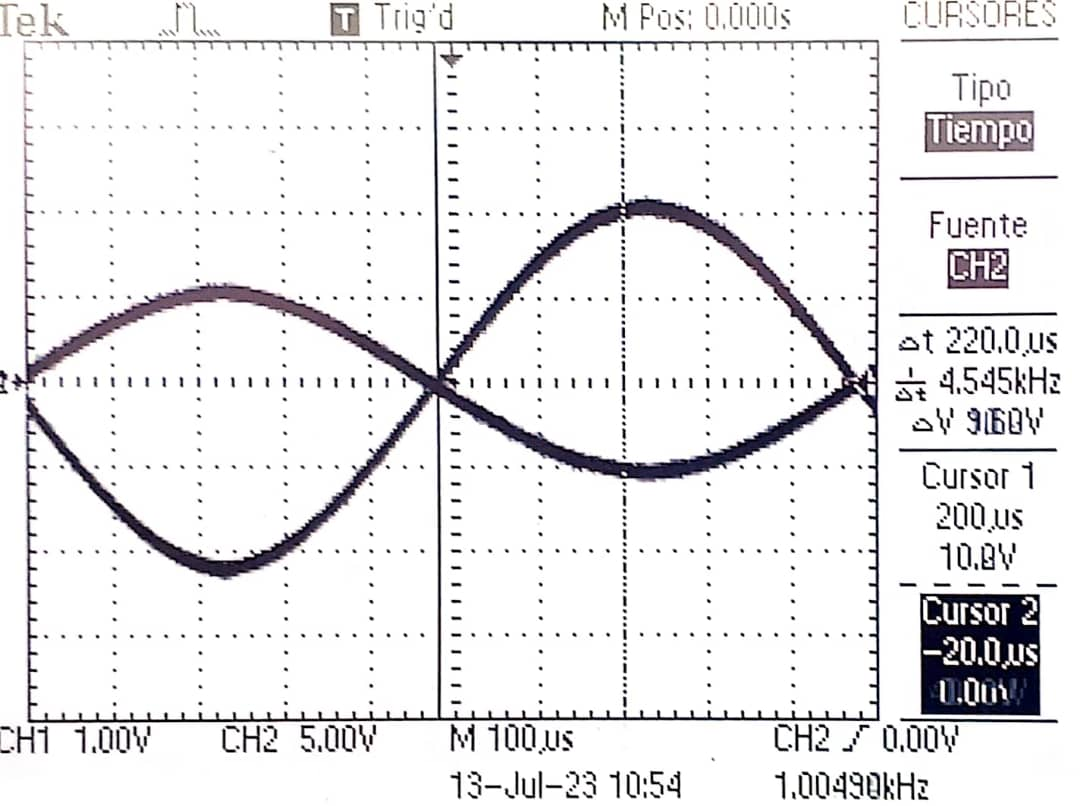
\includegraphics[width=12cm,height=8cm]{Img/q6-1}\\
		\textit{Figura 1. $f = 1kHz$}\\
		
		\vspace{3cm}
		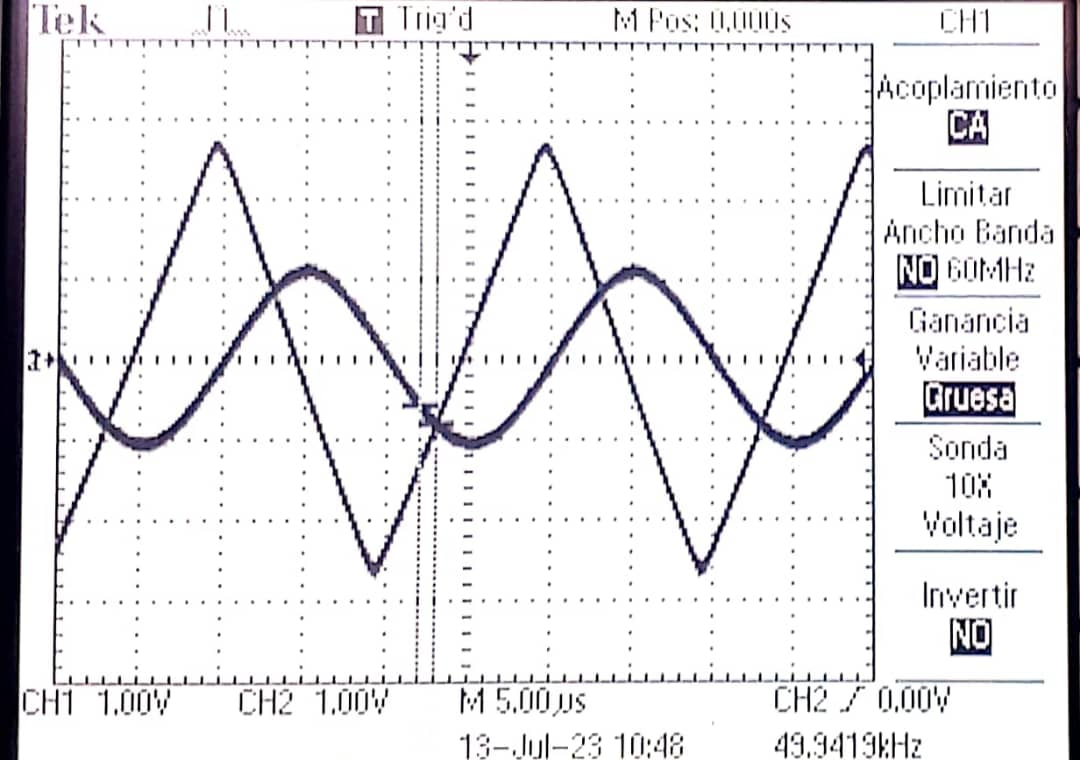
\includegraphics[width=12cm,height=8cm]{Img/q6-2}\\
		\textit{Figura 2. $f = 50kHz$}\\
	\end{center}

	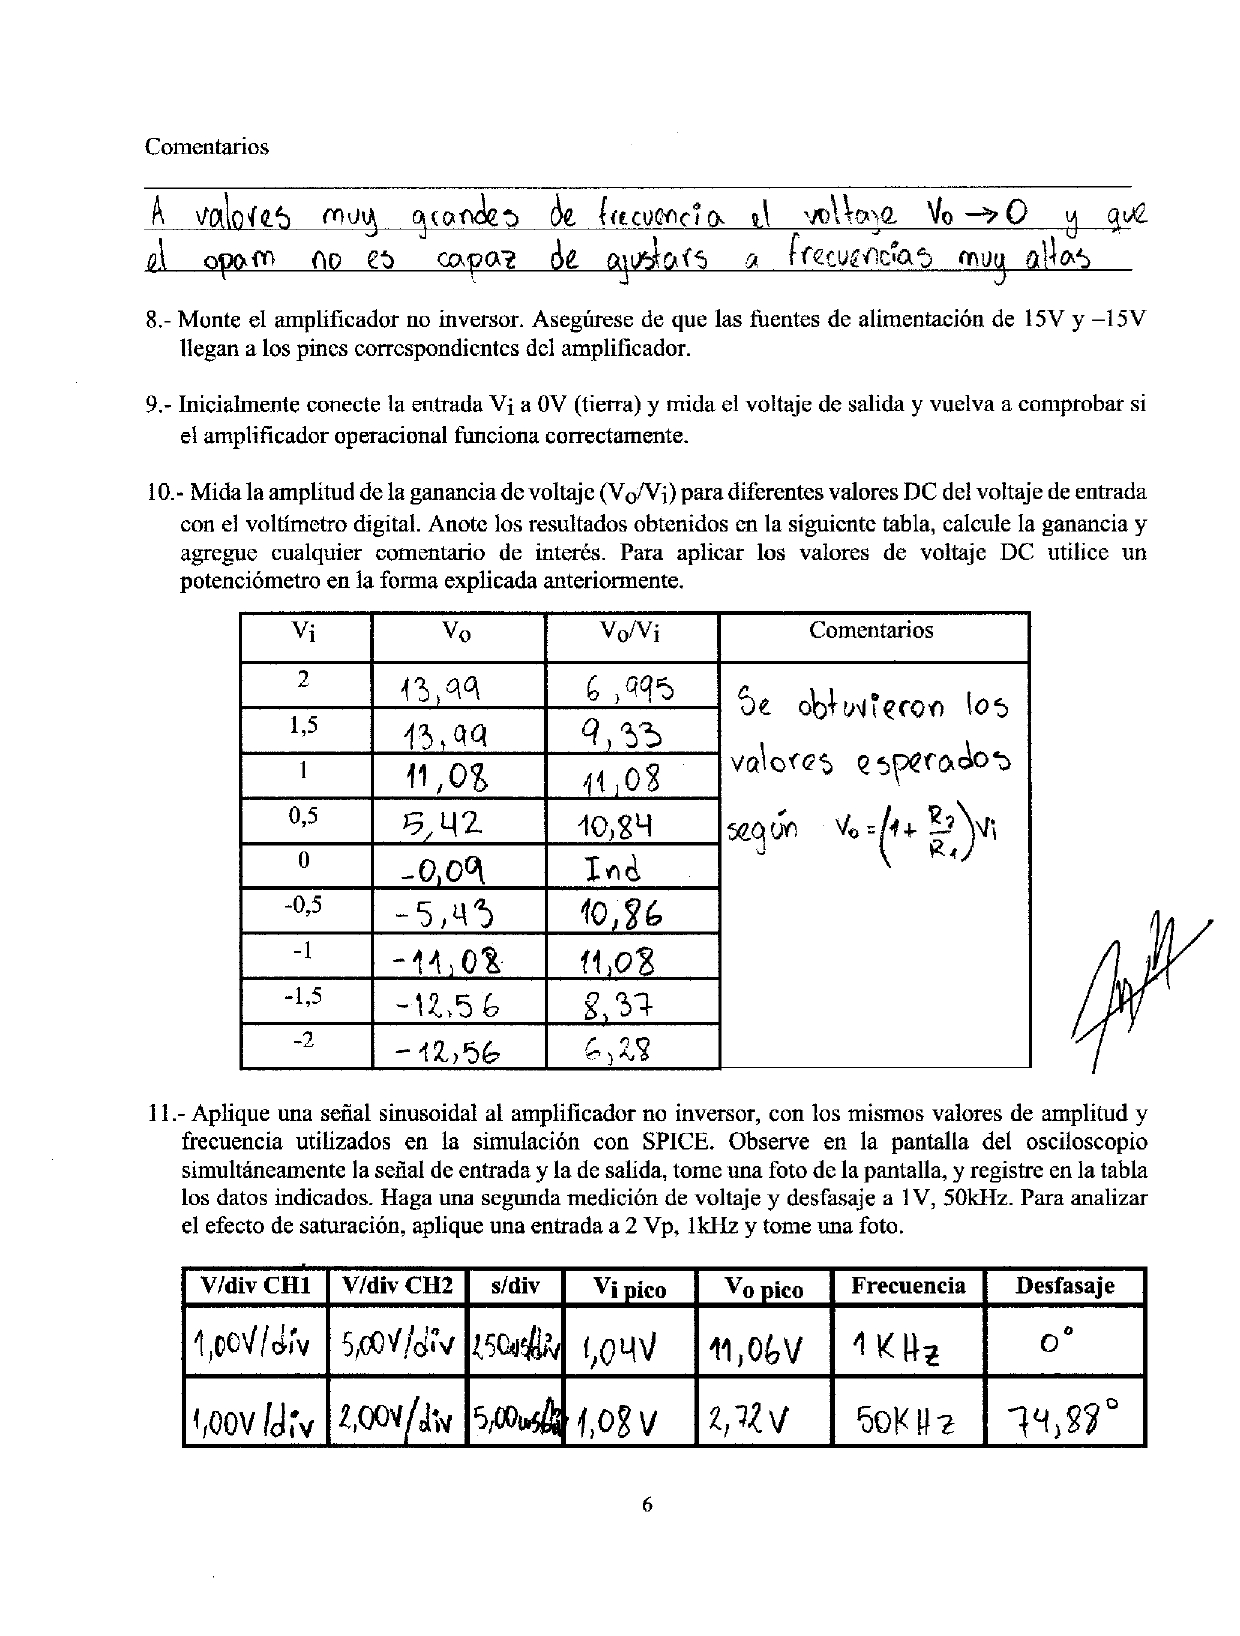
\includegraphics[width=16cm,height=21cm]{Img/lab_9_page-0003}\\
	
	\begin{center}
		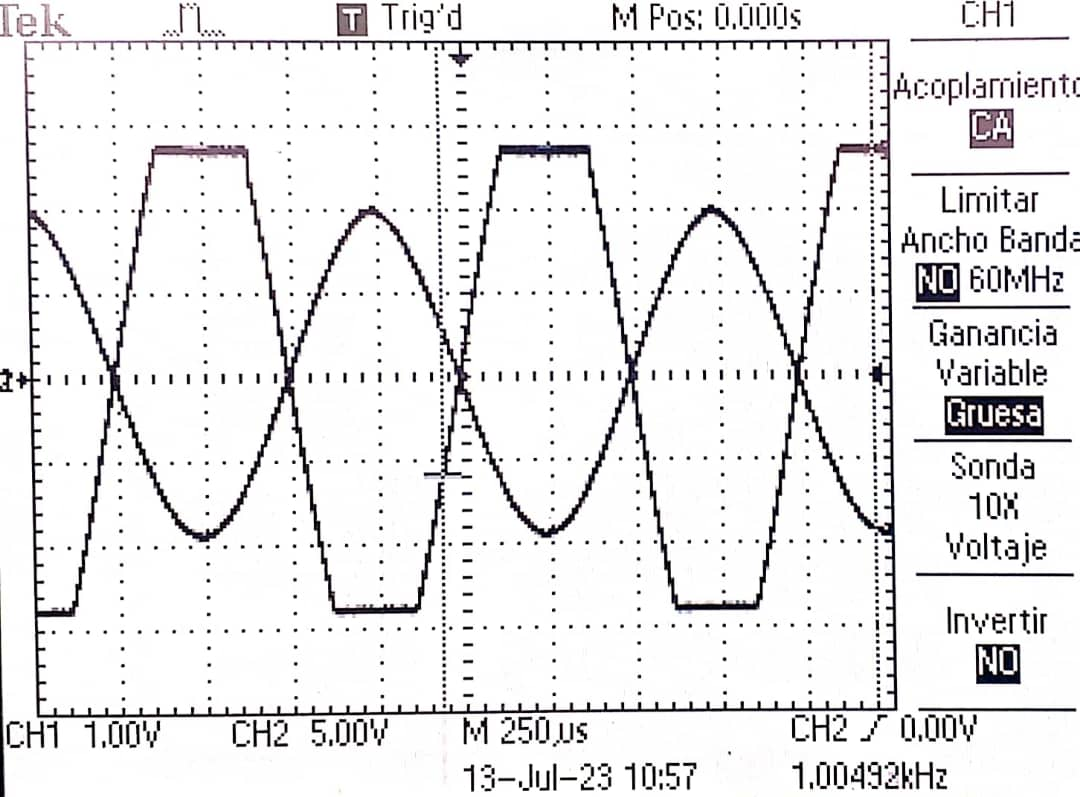
\includegraphics[width=12cm,height=8cm]{Img/q11-1}\\
		\textit{Figura 3. $f = 1kHz$}\\
		
		\vspace{3cm}
		
	\end{center}

	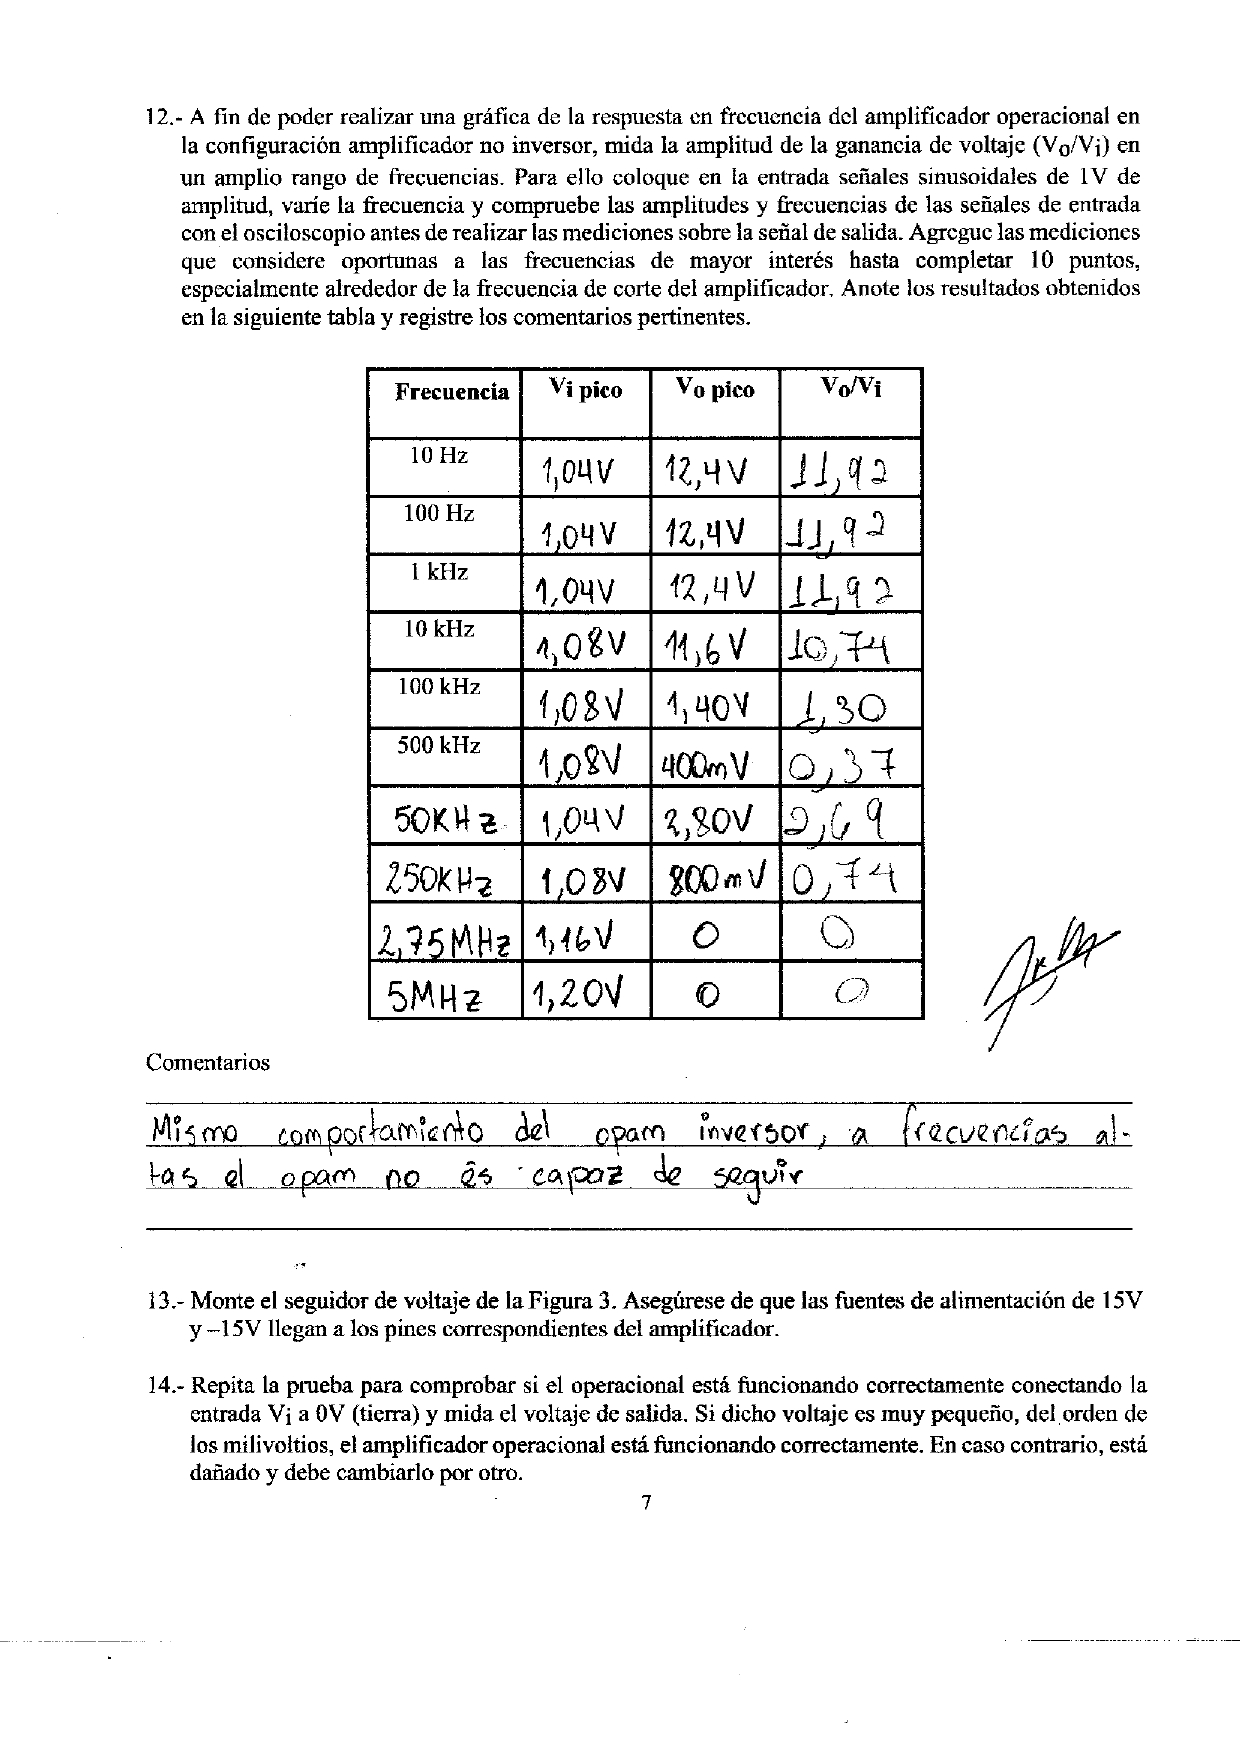
\includegraphics[width=16cm,height=21cm]{Img/lab_9_page-0004}\\
	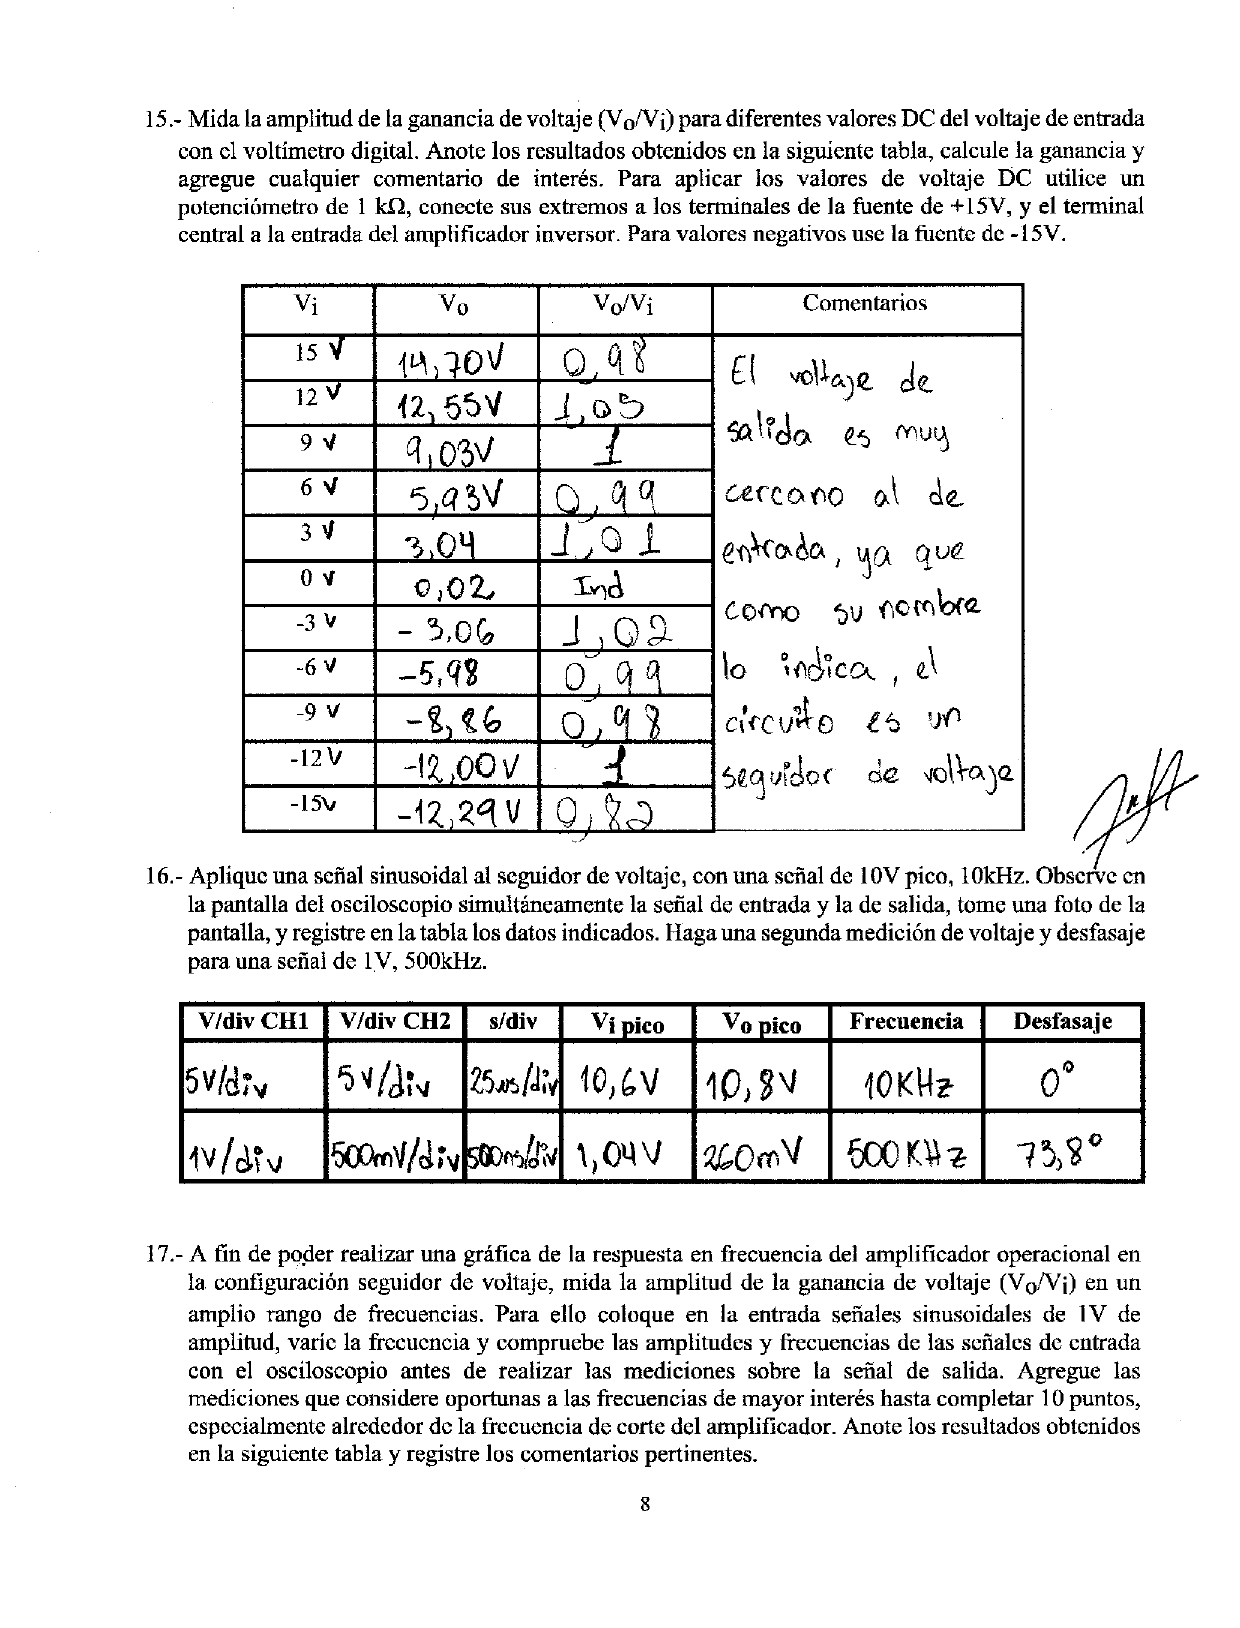
\includegraphics[width=16cm,height=21cm]{Img/lab_9_page-0005}\\
	
	\begin{center}
		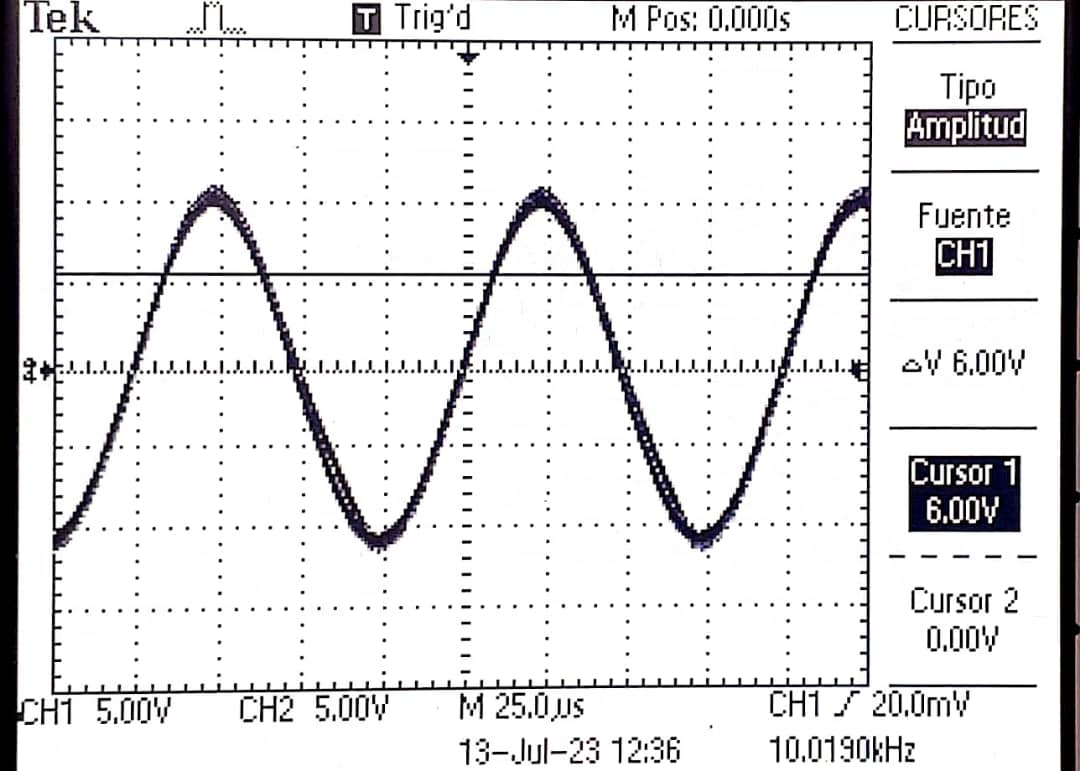
\includegraphics[width=12cm,height=8cm]{Img/q17-1}\\
		\textit{Figura 4. $f = 1kHz$}\\
		
		\vspace{3cm}
		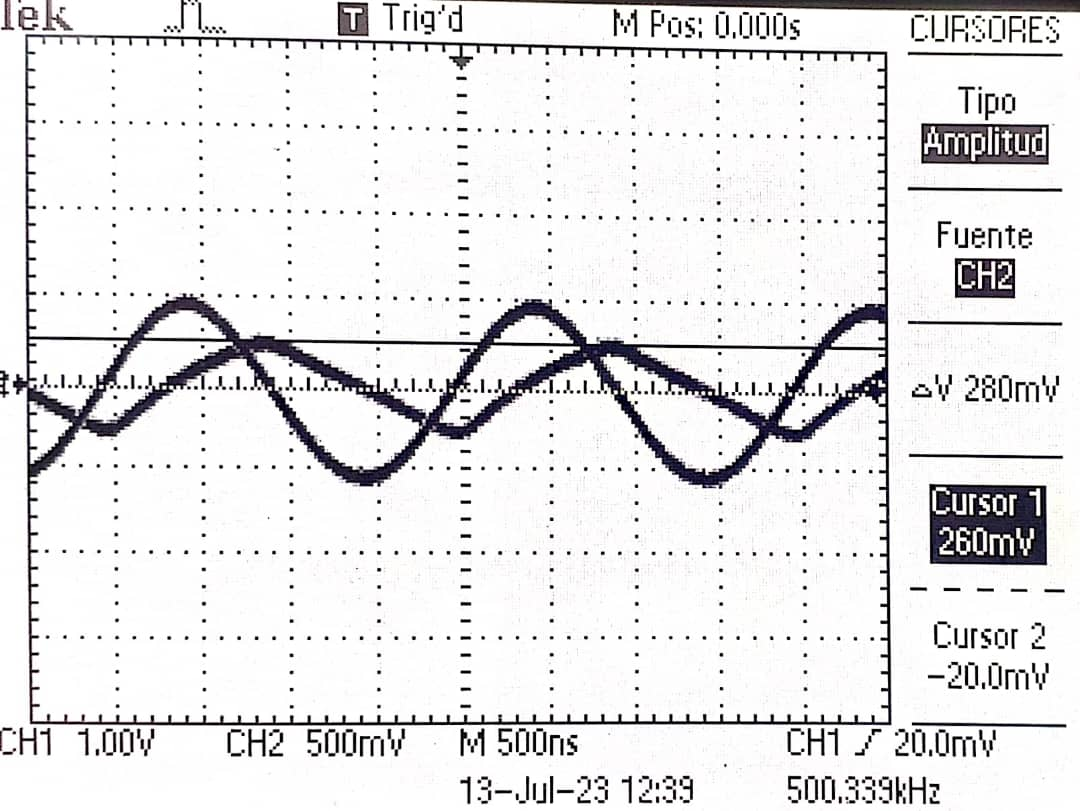
\includegraphics[width=12cm,height=8cm]{Img/q17-2}\\
		\textit{Figura 5. $f = 50kHz$}\\
	\end{center}

	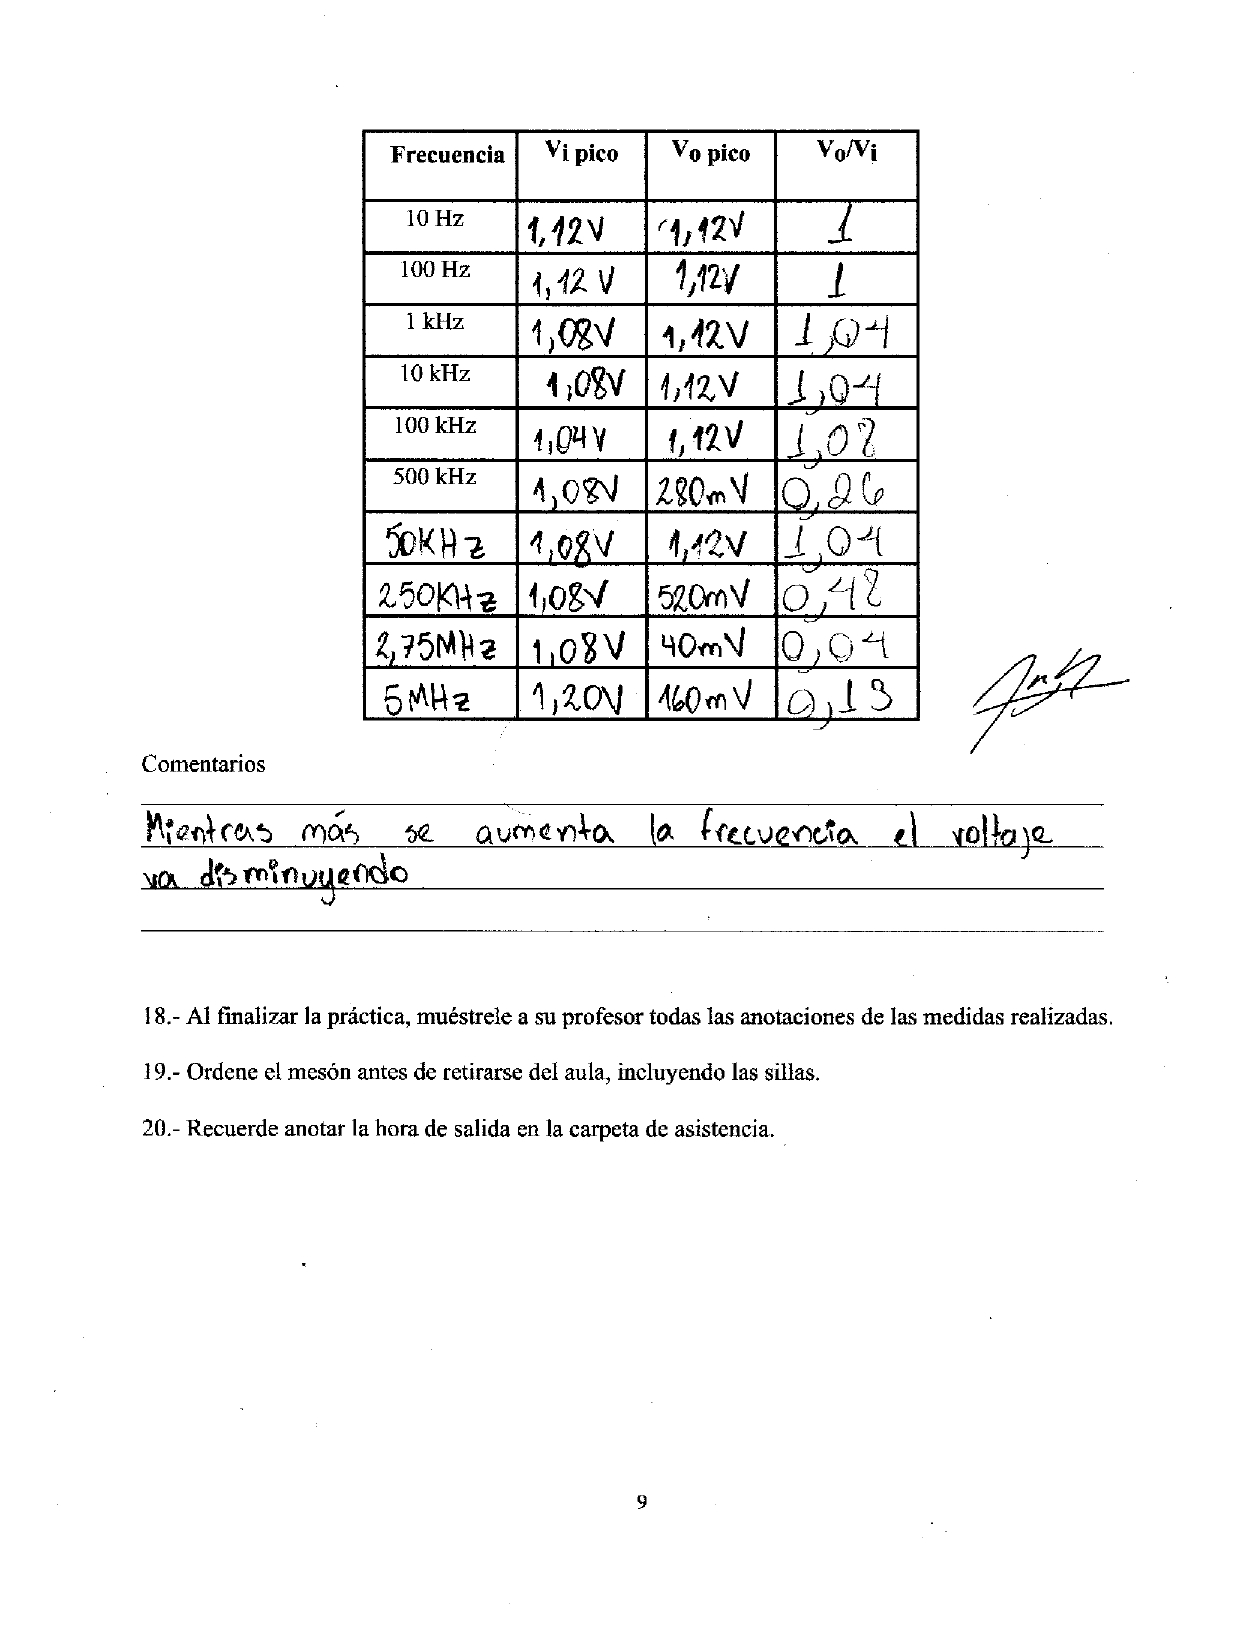
\includegraphics[width=16cm,height=21cm]{Img/lab_9_page-0006}\\
	
	Además, se incluyen las siguientes gráficas:\\
	
	a) Para el amplificador inversor , el voltaje de salida Vo vs. el voltaje de entrada Vi (función de transferencia), e indique sobre la gráfica la zona lineal y la zona de saturación.\\
	
	\begin{center}
		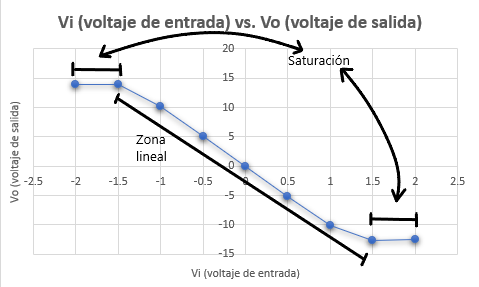
\includegraphics[width=12cm,height=8cm]{Img/graf1}\\
		\textit{Figura 6. Amplificador operacional inversor}\\
	\end{center}
	
	b) Para el amplificador inversor, la amplitud de la ganancia de voltaje, Vo/Vi, vs la frecuencia de operación, f, en escala logarítmica de por lo menos 5 décadas. Identifique sobre la gráfica el ancho de banda.\\
	
	\begin{center}
		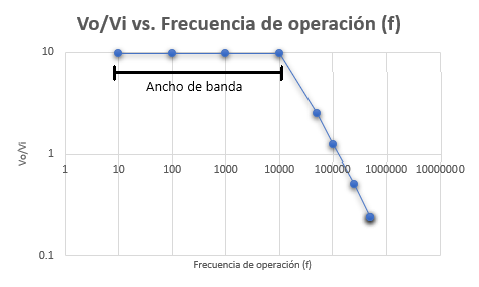
\includegraphics[width=12cm,height=8cm]{Img/graf2}\\
		\textit{Figura 7. Amplificador operacional inversor}\\
	\end{center}
	
	\vspace{3cm}
	c) Para el amplificador no inversor , el voltaje de salida Vo vs. el voltaje de entrada Vi (función de transferencia), e indique sobre la gráfica la zona lineal y la zona de saturación.\\
	
	\begin{center}
		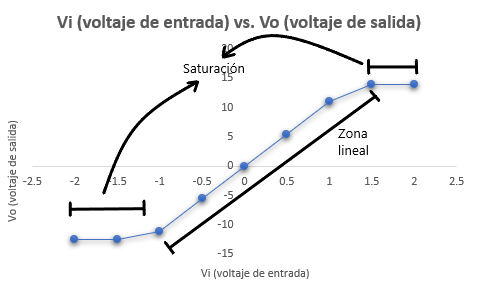
\includegraphics[width=12cm,height=8cm]{Img/graf3}\\
		\textit{Figura 8. Amplificador operacional no inversor}\\
	\end{center}
	
	d) Para el amplificador no inversor, la amplitud de la ganancia de voltaje, Vo/Vi, vs la frecuencia de operación, f, en escala logarítmica de por lo menos 5 décadas. Identifique sobre la gráfica el ancho de banda.\\
	
	\begin{center}
		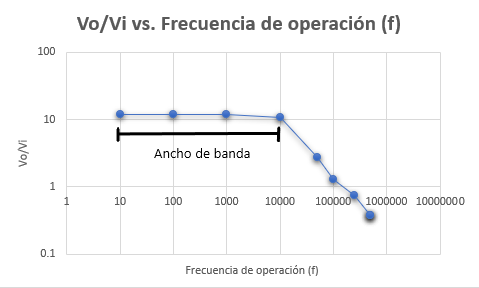
\includegraphics[width=12cm,height=8cm]{Img/graf4}\\
		\textit{Figura 9. Amplificador operacional no inversor}\\
	\end{center}
	
	\vspace{3cm}
	e) Para el seguidor de voltaje, el voltaje de salida Vo vs. el voltaje de entrada Vi (función de transferencia), e indique sobre la gráfica la zona lineal y la zona de saturación.\\
	
	\begin{center}
		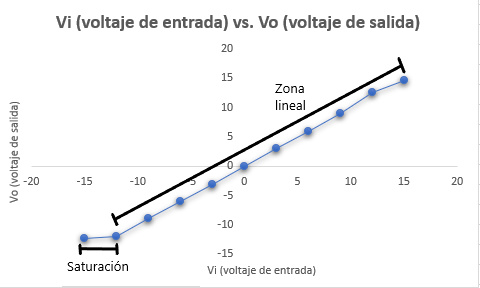
\includegraphics[width=12cm,height=8cm]{Img/graf5}\\
		\textit{Figura 10. Amplificador operacional seguidor de voltaje}\\
	\end{center}
	
	f) Para el seguidor de voltaje, la amplitud de la ganancia de voltaje, Vo/Vi, vs la frecuencia de operación, f, en escala logarítmica de por lo menos 5 décadas. Identifique el ancho de banda.\\
	
	\begin{center}
		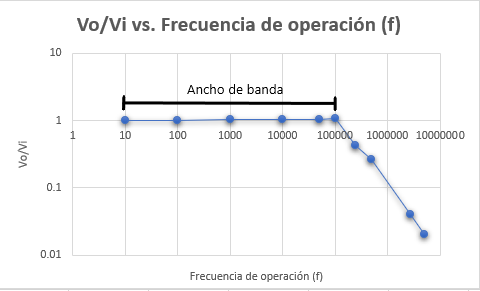
\includegraphics[width=12cm,height=8cm]{Img/graf6}\\
		\textit{Figura 11. Amplificador operacional seguidor de voltaje}\\
	\end{center}
	
	\newpage
	
	\begin{center}
		\textbf{\large ANÁLISIS DE RESULTADOS}\\
	\end{center}
	
	\noindent \textbf{a)} Analice la gráfica de la función de transferencia del amplificador inversor, explicando las zonas que pueden observarse, indicando las razones por las cuales se presenta la saturación y justificando el valor del voltaje máximo obtenido, tanto positivo como	negativo. Compare la ganancia DC obtenida experimentalmente con la teórica y, tomando en cuenta la tolerancia de los componentes utilizados, explique las discrepancias y calcule el error porcentual.\\
	
	Para analizar la gráfica de la función de transferencia del amplificador inversor, observamos que hay dos zonas claramente definidas: una zona lineal y una zona de saturación. En la zona lineal, la ganancia es alta y estable, y sigue la relación de la ganancia teórica del amplificador inversor $(-R_{f}/R_{i})$, donde $R_{f}$ es la resistencia de retroalimentación y $R_{i}$ es la resistencia de entrada. Esto ocurre cuando el amplificador está trabajando dentro de sus limitaciones y no está saturado.\\
	
	En la zona de saturación, la ganancia se reduce significativamente y el amplificador no puede amplificar la señal de manera lineal debido a que la salida alcanza el límite máximo permitido por la fuente de alimentación. Esta zona se produce cuando la señal de entrada es demasiado grande y excede la capacidad de amplificación del amplificador.\\
	
	La comparación entre la ganancia DC obtenida experimentalmente y la teórica puede mostrar discrepancias debido a tolerancias en los valores nominales de las resistencias y a las imperfecciones de los componentes utilizados. El cálculo del error porcentual permitirá cuantificar las diferencias entre los valores teóricos y experimentales.\\
	
	\begin{center}
		\begin{tabular}{|c|c|c|}
			\hline
			Ganancia DC experimental & Ganancia DC teórico & Error porcentual \\
			\hline
			10,06 & 10 & 0,6\% \\
			\hline
		\end{tabular}
	\end{center}
	
	\noindent \textbf{b)} Compare la gráfica obtenida con el análisis TRANSIENT de SPICE para el amplificador inversor con la que Ud. obtuvo en la pantalla del osciloscopio, y explique las discrepancias en cuanto a los valores de la magnitud de voltaje y el desfasaje,	tomando en cuenta la tolerancia de los componentes utilizados. Calcule el error porcentual del voltaje de salida, tomando como referencia el valor teórico.\\
	
	Al comparar la gráfica obtenida en el análisis TRANSIENT de SPICE para el amplificador inversor con la que se obtuvo en la pantalla del osciloscopio, es común encontrar discrepancias en los valores de magnitud de voltaje y desfasaje. Estas discrepancias pueden deberse a las diferencias entre los modelos ideales utilizados en SPICE y el comportamiento real del amplificador operacional en el protoboard. Además, las tolerancias en los componentes utilizados también pueden contribuir a estas diferencias.\\
	
	\begin{center}
		\begin{tabular}{|c|c|c|}
			\hline
			$V_{o}$ experimental & $V_{o}$ teórico & Error porcentual \\
			\hline
			-10,06V & -10V & 0,6\% \\
			\hline
		\end{tabular}
	\end{center}
	
	\noindent \textbf{c)} Para el amplificador inversor, analice los valores del desfasaje entre Vo y Vi correspondientes a las dos frecuencias para las que se realizaron mediciones de desfasaje y comente estos resultados.\\
	
	Los valores del desfasaje entre Vo y Vi correspondientes a las dos frecuencias para las que se realizaron mediciones de desfasaje pueden proporcionar información sobre la fase de la señal amplificada en relación con la señal de entrada. Cuando el desfasaje es cercano a cero grados, significa que la señal de salida está en fase con la señal de entrada. Y cuando el desfasaje es cercano a 180 grados, significa que la señal de salida está en fase opuesta (180 grados fuera de fase) con la señal de entrada.\\
	
	\noindent \textbf{d)} Para el amplificador inversor, compare la gráfica de la amplitud de la ganancia de voltaje Vo/Vi vs la frecuencia de operación que Ud. realizó a partir de los datos medidos en el laboratorio con la obtenida con SPICE mediante el análisis AC SWEEP y explique las discrepancias en cuanto a los valores de la magnitud de voltaje y la frecuencia de corte, tomando en cuenta la tolerancia de los componentes utilizados.\\
	
	Al comparar la gráfica de la amplitud de la ganancia de voltaje (Vo/Vi) vs. frecuencia de operación del amplificador inversor obtenida a partir de los datos medidos en el laboratorio con la obtenida mediante el análisis AC SWEEP en SPICE, es común encontrar discrepancias en los valores de magnitud de voltaje y frecuencia de corte. Al igual que en el análisis TRANSIENT, estas diferencias pueden deberse a las tolerancias de los componentes y a las limitaciones del amplificador operacional en el protoboard.\\
	
	\noindent \textbf{e)} Analice la gráfica de la función de transferencia del amplificador no inversor, explicando las zonas que pueden observarse, indicando las razones por las cuales se presenta la saturación y justificando el valor del voltaje máximo obtenido, tanto positivo como negativo. Compare la ganancia DC obtenida experimentalmente con la teórica y, tomando en cuenta la tolerancia de los componentes utilizados, explique las discrepancias y calcule el error porcentual.\\
	
	Para analizar la gráfica de la función de transferencia del amplificador no inversor, se aplican consideraciones similares a las del amplificador inversor. Se observan zonas lineales y de saturación, y el valor máximo de voltaje, tanto positivo como negativo, está determinado por la tensión de alimentación.\\
	
	\begin{center}
		\begin{tabular}{|c|c|c|}
			\hline
			Ganancia DC experimental & Ganancia DC teórico & Error porcentual \\
			\hline
			11,08 & 11 & 0,73\% \\
			\hline
		\end{tabular}
	\end{center}
	
	\noindent \textbf{f)} Compare la gráfica obtenida con el análisis TRANSIENT de SPICE para el amplificador no inversor con la que Ud. obtuvo en la pantalla del osciloscopio, y explique las discrepancias en cuanto a los valores de la magnitud de voltaje y el desfasaje, tomando en cuenta la tolerancia de los componentes utilizados. Calcule el error porcentual del voltaje de salida, tomando como referencia el valor teórico.\\
	
	Al comparar la gráfica obtenida en el análisis TRANSIENT de SPICE para el amplificador no inversor con la que se obtuvo en la pantalla del osciloscopio, es común encontrar discrepancias en los valores de magnitud de voltaje y desfasaje debido a las mismas razones mencionadas anteriormente, como las diferencias entre los modelos teóricos y el comportamiento real del circuito en el protoboard.\\
	
	\begin{center}
		\begin{tabular}{|c|c|c|}
			\hline
			$V_{o}$ experimental & $V_{o}$ teórico & Error porcentual \\
			\hline
			11,08V & 11V & 0,73\% \\
			\hline
		\end{tabular}
	\end{center}
	
	\noindent \textbf{g)} Para el amplificador no inversor, analice los valores del desfasaje entre Vo y Vi correspondientes a las dos frecuencias para las que se realizaron mediciones de desfasaje y comente estos resultados.\\
	
	Los valores del desfasaje entre Vo y Vi correspondientes a las dos frecuencias para las que se realizaron mediciones de desfasaje proporcionarán información sobre la fase de la señal amplificada en relación con la señal de entrada, al igual que en el amplificador inversor.
	
	\noindent \textbf{h)} Para el amplificador no inversor, compare la gráfica de la amplitud de la ganancia de voltaje Vo/Vi vs la frecuencia de operación que Ud. realizó a partir de los datos	medidos en el laboratorio con la obtenida con SPICE mediante el análisis AC SWEEP y explique las discrepancias en cuanto a los valores de la magnitud de voltaje y la frecuencia de corte, tomando en cuenta la tolerancia de los componentes utilizados.\\
	
	Al comparar la gráfica de la amplitud de la ganancia de voltaje (Vo/Vi) vs. frecuencia de operación del amplificador no inversor obtenida a partir de los datos medidos en el laboratorio con la obtenida mediante el análisis AC SWEEP en SPICE, se pueden encontrar discrepancias en los valores de magnitud de voltaje y frecuencia de corte debido a las tolerancias de los componentes y las limitaciones del protoboard.\\
	
	\noindent \textbf{i)} Analice la gráfica de la función de transferencia del seguidor de voltaje, explicando	las zonas que pueden observarse, indicando las razones por las cuales se presenta la saturación y justificando el valor del voltaje máximo obtenido, tanto positivo como	negativo. Compare la ganancia DC obtenida experimentalmente con la teórica y, tomando en cuenta la tolerancia de los componentes utilizados, explique las discrepancias y calcule el error porcentual.\\
	
	Para analizar la gráfica de la función de transferencia del seguidor de voltaje, se aplican consideraciones similares a las de los amplificadores anteriores. Se observan zonas lineales y de saturación, y el valor máximo de voltaje, tanto positivo como negativo, está determinado por la tensión de alimentación.\\
	
	\begin{center}
		\begin{tabular}{|c|c|c|}
			\hline
			Ganancia DC experimental & Ganancia DC teórico & Error porcentual \\
			\hline
			1,05 & 1 & 5\% \\
			\hline
		\end{tabular}
	\end{center}
	
	\noindent \textbf{j)} Compare la gráfica obtenida con el análisis TRANSIENT de SPICE para el seguidor de voltaje con la que Ud. obtuvo en la pantalla del osciloscopio y explique las discrepancias en cuanto a los valores de la magnitud de voltaje y el desfasaje, tomando	en cuenta la tolerancia de los componentes utilizados. Calcule el error porcentual del	voltaje de salida, tomando como referencia el valor teórico.\\
	
	Al comparar la gráfica obtenida en el análisis TRANSIENT de SPICE para el seguidor de voltaje con la que se obtuvo en la pantalla del osciloscopio, es común encontrar discrepancias en los valores de magnitud de voltaje y desfasaje debido a las mismas razones mencionadas anteriormente, como las diferencias entre los modelos teóricos y el comportamiento real del circuito en el protoboard.\\
	
	\begin{center}
		\begin{tabular}{|c|c|c|}
			\hline
			$V_{o}$ experimental & $V_{o}$ teórico & Error porcentual \\
			\hline
			12,55V & 12V & 4,58\% \\
			\hline
		\end{tabular}
	\end{center}
	
	\noindent \textbf{k)} Para el seguidor de voltaje, analice los valores del desfasaje entre Vo y Vi	correspondientes a las dos frecuencias para las que se realizaron mediciones de desfasaje y comente estos resultados.\\
	
	Los valores del desfasaje entre Vo y Vi correspondientes a las dos frecuencias para las que se realizaron mediciones de desfasaje proporcionarán información sobre la fase de la señal amplificada en relación con la señal de entrada, al igual que en los amplificadores anteriores.\\
	
	\noindent \textbf{l)} Para el seguidor de voltaje, compare la gráfica de la amplitud de la ganancia de voltaje,	Vo/Vi vs la frecuencia de operación que Ud. realizó a partir de los datos medidos en el laboratorio con la obtenida con SPICE mediante el análisis AC SWEEP y explique las discrepancias en cuanto a los valores de la magnitud de voltaje y la frecuencia de corte, considerando el valor teórico de dicha frecuencia.\\
	
	Al comparar la gráfica de la amplitud de la ganancia de voltaje (Vo/Vi) vs. frecuencia de operación del seguidor de voltaje obtenida a partir de los datos medidos en el laboratorio con la obtenida mediante el análisis AC SWEEP en SPICE, se pueden encontrar discrepancias en los valores de magnitud de voltaje y frecuencia de corte debido a las tolerancias de los componentes y las limitaciones del protoboard. Considerando el valor teórico de la frecuencia de corte, se pueden identificar las diferencias en las respuestas en frecuencia.\\
	
	\noindent \textbf{m)} Comente sobre las formas de onda obtenidas al aplicar una entrada de 2V, 1kHz tanto para el amplificador inversor como para el no inversor.\\
	
	Se puede observar cómo la señal se invierte y amplifica en el amplificador inversor, mientras que en el no inversor, la señal se amplifica sin invertirse.\\
	
	En el caso del amplificador inversor, las diferencias en las amplitudes de las formas de onda pueden atribuirse a varios factores. En primer lugar, los amplificadores operacionales reales, como el UA741, tienen limitaciones en su rendimiento y no son ideales. Estas limitaciones pueden incluir ganancia finita, ancho de banda limitado, corriente de polarización y resistencias internas. Estas imperfecciones afectan el comportamiento real del amplificador y pueden desviar los resultados experimentales de los cálculos teóricos.\\
	
	Además, las tolerancias de los componentes utilizados, como las resistencias, también pueden contribuir a las diferencias en las amplitudes de las formas de onda. Pequeñas variaciones en los valores reales de las resistencias pueden tener un efecto significativo en la ganancia del amplificador inversor, ya que la ganancia depende directamente de los valores de resistencia utilizados en el circuito.\\
	
	Similarmente, para el amplificador no inversor, las diferencias en las amplitudes de las formas de onda también pueden deberse a las mismas razones mencionadas anteriormente, como las limitaciones del amplificador operacional real y las tolerancias de los componentes.\\
	
	Es importante destacar que las diferencias entre las ganancias teóricas y experimentales no implican necesariamente una falla en el diseño o en el funcionamiento del circuito. Como se mencionó anteriormente, los amplificadores operacionales reales tienen limitaciones que afectan su comportamiento y, por lo tanto, es normal esperar algunas discrepancias entre los resultados teóricos y experimentales.\\
	
	\newpage
	
	\begin{center}
		\textbf{\large CONCLUSIONES}\\
	\end{center}
	
	En la práctica realizada, se llevaron a cabo diversas configuraciones utilizando el amplificador operacional UA741, incluyendo el amplificador inversor, el amplificador no inversor y el seguidor de voltaje. Se analizaron las características más resaltantes de cada circuito, así como su respuesta en frecuencia.\\
	
	En cuanto a los procedimientos, se montaron los circuitos en un protoboard siguiendo las especificaciones dadas en el enunciado de la práctica. Se utilizaron resistencias con valores nominales determinados, y se aplicaron diferentes tensiones DC como señal de entrada para cada configuración. Se midieron los voltajes de entrada y salida utilizando un osciloscopio y se registraron los datos necesarios para realizar los análisis posteriores.\\
	
	Los resultados obtenidos mostraron que los amplificadores operacionales UA741 son dispositivos versátiles y ampliamente utilizados en aplicaciones electrónicas. Se observaron las zonas lineales y de saturación en las gráficas de voltaje de salida versus voltaje de entrada para cada configuración.\\
	
	En el amplificador inversor, se confirmó su comportamiento inversor y su ganancia DC fue consistente con la ganancia teórica $(-R_{f}/R_{i})$. Se identificaron las zonas lineales y de saturación, y se analizó la razón detrás de la saturación. Las discrepancias entre la ganancia DC teórica y experimental se explicaron mediante el cálculo del error porcentual, considerando las tolerancias de los componentes.\\
	
	En el análisis comparativo entre las gráficas obtenidas en el osciloscopio y las simulaciones en SPICE, se observaron algunas diferencias, atribuibles a las simplificaciones en los modelos utilizados en SPICE y a las limitaciones en el protoboard. También se analizó el desfasaje entre la señal de entrada y salida.\\
	
	En el amplificador no inversor, se confirmó su comportamiento no inversor y su ganancia DC fue acorde con la ganancia teórica $(1 + R_{f}/R_{i})$. Se analizaron las zonas lineales y de saturación, y se justificó el valor de los voltajes máximos de salida. Las discrepancias entre la ganancia DC teórica y experimental se analizaron mediante el cálculo del error porcentual, considerando las tolerancias de los componentes.\\
	
	En conclusión, la práctica proporcionó una comprensión práctica de las características y comportamientos de los amplificadores operacionales en diferentes configuraciones. Se observaron las zonas lineales y de saturación, y se identificaron las limitaciones de cada circuito. Las diferencias entre los resultados teóricos y experimentales se atribuyeron a las tolerancias de los componentes y las imperfecciones del protoboard. La práctica permitió fortalecer los conocimientos sobre amplificadores operacionales y su aplicación en circuitos electrónicos.\\
	
	\newpage
	
	\begin{center}
		\textbf{\large BIBLIOGRAFÍA}\\
	\end{center}
	
	\noindent 1.- Laboratorios de Circuitos Electrónicos, Guía Teórica versión electrónica, ubicada en la página web de laboratorio C, http://www.labc.usb.ve, enlace a "Páginas web de Asignaturas", EC1281- Laboratorio de Mediciones Eléctricas 2013\\
	
	\noindent 2.- Análisis básico de Circuitos Eléctricos, Quinta Edición. Johnson, Hilburn, Johnson y Scott. Prentice Hall.\\
	
	\noindent 3.- Introduction to Electric Circuits. Dorf. Wiley.
	
\end{document}
